\documentclass[letterpaper,10pt]{book}
% Change to 10 pt
\usepackage{pdfpages}
\usepackage{morewrites}			% to counteract the no write space problem
\setcounter{tocdepth}{6}

\usepackage[framemethod=TikZ]{mdframed}

\usepackage{fancyhdr}

\usepackage{paralist}
\usepackage{amsmath}
\usepackage{amsfonts}
\usepackage{amssymb}
\usepackage{graphicx}

\usepackage{datetime}
%\usepackage{ulem}

%\usepackage[nottoc]{toobibind}

\usepackage[inline]{enumitem}

% Outer margin at 2.50 is exacty correct to fit the ``corruption alert'' tables
\usepackage[inner=1.0in, outer=2.50in, top=2.54cm,bottom=2.54cm, marginparwidth=2.25in]{geometry}

\usepackage{marginnote}
\usepackage{longtable}
\usepackage{booktabs}
\usepackage{xcolor}

\usepackage{soul}

%%%%%%%%%%%%
\definecolor{ForestGreen}{rgb}{0.00,0.29,0.098}
%%%%%%%%%%%%

\usepackage{marginnote}

\usepackage{imakeidx} 
\usepackage[
	backref=true,
	style=numeric,
%	citestyle=numeric,
	backend=bibtex
	]{biblatex}
\usepackage[driverfallback=hypertex,colorlinks=True]{hyperref}
\usepackage{cleveref}

\makeindex[name=scripture,columnsep=20pt, columnseprule=True,columns=3, title=Scripture References]
\makeindex[name=speaker,columnsep=20pt, columnseprule=True,,columns=2, title=Sermon Creator]
\makeindex[name=series,columnsep=20pt, columnseprule=True,,columns=2, title=Sermon Series]
\makeindex[name=date,columnsep=20pt, columnseprule=True,columns=2, title=Sermon Date]
\makeindex[name=event,columnsep=20pt, columnseprule=True,columns=2, title=Event]
\makeindex[name=topic,columnsep=20pt, columnseprule=True,columns=2, title=Topic]
\makeindex[name=AWIP,columnsep=20pt, columnseprule=True,columns=3, title=All Words in Passage]
\makeindex[name=NWIV,columnsep=20pt, columnseprule=True,columns=3, title=Number of Words in Verse]
\makeindex[name=PNIP,columnsep=20pt, columnseprule=True,columns=3, title=Proper Names in Passage]
\makeindex[name=PEIP,columnsep=20pt, columnseprule=True,columns=2, title=Prophetic Events in Passage]
\makeindex[name=TWPAQ,columnsep=20pt, columnseprule=True,columns=1, title=13-Word Phrases and Quotes]
\makeindex[name=PFTTIS,columnsep=20pt, columnseprule=False,columns=3, title=Phrases found 13 times in scripture]
\makeindex[name=WFTTIS,columnsep=20pt, columnseprule=False,columns=3, title=Words found 13 times in scripture]
\makeindex[name=WFITV,columnsep=20pt, columnseprule=False,columns=3, title=Words found in exactly 13 verses]
\makeindex[name=EVENTS,columnsep=20pt, columnseprule=False,columns=2, title=Sermon Log by Place]
\makeindex[name=QUESTIONS,columnsep=20pt, columnseprule=False,columns=2, title=Bible Questions]
\makeindex[name=DOCTRINES,columnsep=20pt, columnseprule=False,columns=2, title=Doctrines]
\makeindex[name=SONGS,columnsep=20pt, columnseprule=False,columns=1, title=Songs]
\makeindex[name=LOCATION,columnsep=20pt, columnseprule=False,columns= 2, title=Location]
\makeindex[name=FACEBOOK,columnsep=20pt, columnseprule=False,columns=2, title=Facebook]
\makeindex[name=DEVOTIONAL,columnsep=20pt, columnseprule=False,columns=2, title=Devotional Items]
%%%%%%%%%%%%%%%%% EXTRA COLORS
\definecolor{champagne}{rgb}{0.97,0.91,0.81}
\definecolor{bone}{rgb}{0.89,0.85,0.79}
\pagestyle{fancy}
\fancyhf{}
\fancyhead[LE,RO]{\today}
\fancyhead[RE,LO]{Daily Bible Reading}
\fancyhead[CE,CO]{-page \thepage  - }

\fancyfoot[CO,CE]{\leftmark}
%\fancyfoot[LE,RO]{CSCE 692, HW1}

\title{DBR\\
Daily \\ Reads}
\author{Keith Anthony \\
\today }
%+/ffffff +   \pagenumbering{gobble}
\bibliography{Bibliographies/All20220122}

\setlength{\fboxsep}{1.0pt}

\usepackage[utf8]{inputenc}
\usepackage{tikz}

\begin{document}
%%%%%%%%%%%% Tile Page

\begin{titlepage}

\begin{flushright}
\rightskip=-2.5cm
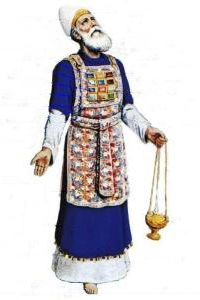
\includegraphics[width=50mm,scale=1.5]{Extras/Melchisedec.jpg}
\vspace{0.4in}  % Create a title for the document and write it in bold font
\LARGE{\textbf{\date}} % Again, do a line break
\linebreak 
% Create a subtitle \large{with Outlines, Statistics, Cross References, and Notes}
\vspace{0.5in}
\begin{flushleft}
\LARGE{Day \#48: Thursday, 17 February 2022 PLAIN\\} \vspace{0.25in}
\LARGE{Numbers 22-24 Psalm 48 Proverb 17}
\end{flushleft}
\vspace{0.6in}
\bigskip

\normalsize{Xenia, Oh.\\}
\normalsize{created: \today}
\vspace{1.3in}

\end{flushright}
\end{titlepage}

\newpage 
\tableofcontents\hypertarget{TOC}{}

\hyphenation{A-bim-e-lech bre-thren E-phra-im  Gib-e-o-nites Jer-u-sa-lem through-out Phil-i-stines The-o-phil-us Am-a-le-kites ven-geance Mesh-el-e-mi-ah onan-ism Phar-a-oh thoughts grev-ous-ness Hach-a-liah adul-ter-er Shad-rach}

%%%%%%%%%%%%%%%%% EXTRA COLORS
%%%%%%%%%%%%%%%%% EXTRA COLORS
%%%%%%%%%%%%%%%%% EXTRA COLORS
\definecolor{champagne}{rgb}{0.97,0.91,0.81}
\definecolor{bone}{rgb}{0.89,0.85,0.79}

\definecolor{ForestGreen}{rgb}{0.00,0.29,0.098}
\definecolor{GIVING}{cmyk}{1,0.0,0.72,.1}

\definecolor{MLPE}{cmyk}{1,1,0,.45}
\definecolor{SOCCER}{cmyk}{.77, 0, .42, .49}
\definecolor{PAYBILL}{cmyk}{0,0.83,0.76,0.07}
\definecolor{SERMON}{cmyk}{.14,.9,0,.30} % aka seance \href{http://www.flatuicolorpicker.com/purple-cmyk-color-model/}{seance}
\definecolor{BIBLE}{cmyk}{0,.17,.74,.17}
\definecolor{WORKBLUE}{cmyk}{1, .5, 0, .6}
\definecolor{myOrange}{cmyk}{0, .4, .98, .03}
\definecolor{myTan}{cmyk}{0.0,.07,.17,.10}
\definecolor{myRed}{cmyk}{0,1,1,0}
\definecolor{myWhite}{cmyk}{0,0,0,0}
\definecolor{BLUESoD}{cmyk}{.97,.84,0,.04}
\definecolor{WHITE}{cmyk}{0,0,0,0}
\definecolor{OLDGOLD}{cmyk}{0.05,0.3,1.00,0}
\definecolor{CASTLETON}{cmyk}{1,0,0.31,0.66}
\definecolor{cadmiumgreen}{rgb}{0.0, 0.42, 0.24}
\definecolor{jungle}{rgb}{0.203,0.4882,0.1718}
\definecolor{MYGOLD}{rgb}{1,.84,0}

\definecolor{MYLIGHTGRAY}{rgb}{.85,.85,.85}

\definecolor{codegreen}{rgb}{0,0.6,0}
\definecolor{codegray}{rgb}{0.5,0.5,0.5}
\definecolor{codepurple}{rgb}{0.58,0,0.82}
\definecolor{backcolour}{rgb}{0.95,0.95,0.92}


\mdfdefinestyle{MyFrame}{%
    linecolor=blue,
    outerlinewidth=2pt,
    roundcorner=5pt,
    innertopmargin=\baselineskip,
    innerbottommargin=\baselineskip,
    innerrightmargin=10pt,
    innerleftmargin=10pt,
    backgroundcolor=gray!25!white}


\mdfdefinestyle{MyFrame2}{%
    linecolor=black,
    outerlinewidth=2pt,
    roundcorner=5pt,
    innertopmargin=\baselineskip,
    innerbottommargin=\baselineskip,
    innerrightmargin=10pt,
    innerleftmargin=10pt,
    backgroundcolor=yellow!25!white}


%%%%%
%% for PFTTIS list
%%%%%

%%% And Joseph said unto
\index[PFTTIS]{And Joseph said unto!Genesis!Gen 40:008}
\index[PFTTIS]{And Joseph said unto!Genesis!Gen 40:012}
\index[PFTTIS]{And Joseph said unto!Genesis!Gen 41:025}
\index[PFTTIS]{And Joseph said unto!Genesis!Gen 42:014}
\index[PFTTIS]{And Joseph said unto!Genesis!Gen 42:018}
\index[PFTTIS]{And Joseph said unto!Genesis!Gen 44:015}
\index[PFTTIS]{And Joseph said unto!Genesis!Gen 45:003}
\index[PFTTIS]{And Joseph said unto!Genesis!Gen 45:004}
\index[PFTTIS]{And Joseph said unto!Genesis!Gen 46:031}
\index[PFTTIS]{And Joseph said unto!Genesis!Gen 48:009}
\index[PFTTIS]{And Joseph said unto!Genesis!Gen 48:018}
\index[PFTTIS]{And Joseph said unto!Genesis!Gen 50:019}
\index[PFTTIS]{And Joseph said unto!Genesis!Gen 50:024}


%%% a shadow
\index[PFTTIS]{a shadow!1Chronicles!1Chr 029:15}
\index[PFTTIS]{a shadow!Job!Job 008:09}
\index[PFTTIS]{a shadow!Job!Job 014:02}
\index[PFTTIS]{a shadow!Job!Job 017:07}
\index[PFTTIS]{a shadow!Psalm!Psa 102:011}
\index[PFTTIS]{a shadow!Psalm!Psa 144:004}
\index[PFTTIS]{a shadow!Ecclesiastes!Eccl 006:012}
\index[PFTTIS]{a shadow!Ecclesiastes!Eccl 008:013}
\index[PFTTIS]{a shadow!Isaiah!Isa 04:006}
\index[PFTTIS]{a shadow!Isaiah!Isa 25:004}
\index[PFTTIS]{a shadow!Jonah!Jnh 04:06}
\index[PFTTIS]{a shadow!Colossians!Col 02:017}
\index[PFTTIS]{a shadow!Hebews!Heb 10:001}

%%% blessed is the man
\index[PFTTIS]{blessed is the man!Psalm!Psa 001:001}
\index[PFTTIS]{blessed is the man!Psalm!Psa 032:002}
\index[PFTTIS]{blessed is the man!Psalm!Psa 034:008}
\index[PFTTIS]{blessed is the man!Psalm!Psa 065:004}
\index[PFTTIS]{blessed is the man!Psalm!Psa 084:005}
\index[PFTTIS]{blessed is the man!Psalm!Psa 084:012}
\index[PFTTIS]{blessed is the man!Psalm!Psa 094:012}
\index[PFTTIS]{blessed is the man!Psalm!Psa 112:001}
\index[PFTTIS]{blessed is the man!Proverbs!Pro 008:034}
\index[PFTTIS]{blessed is the man!Isaiah!Isa 056:002}
\index[PFTTIS]{blessed is the man!Jeremiah!Jer 017:007}
\index[PFTTIS]{blessed is the man!Romans!Rom 004:008}
\index[PFTTIS]{blessed is the man!James!Jam 001:012}


%%% carry them
\index[PFTTIS]{carry them!Leviticus!Lev 14:045}
\index[PFTTIS]{carry them!Numbers!Num 11:012}
\index[PFTTIS]{carry them!Joshua!Jsh 04:003}
\index[PFTTIS]{carry them!1Samuel!1Sam 20:040}
\index[PFTTIS]{carry them!1Kings!1Kng 08:046}
\index[PFTTIS]{carry them!2Chronicles!2Chr 06:036}
\index[PFTTIS]{carry them!Ezra!Ezra 05:015}
\index[PFTTIS]{carry them!Isaiah!Isa 40:011}
\index[PFTTIS]{carry them!Isaiah!Isa 41:016}
\index[PFTTIS]{carry them!Isaiah!Isa 57:013}
\index[PFTTIS]{carry them!Jeremiah!Jer 20:004}
\index[PFTTIS]{carry them!Jeremiah!Jer 20:005}
\index[PFTTIS]{carry them!Jeremiah!Jer 43:012}


\index[PFTTIS]{good tidings!2Samuel!2Sam 18:027}
\index[PFTTIS]{good tidings!1Kings!1Ki 01:042}
\index[PFTTIS]{good tidings!2Kings!2Ki 07:009 (2x)}
\index[PFTTIS]{good tidings!Isaiah!Isa 40:009 (2x)}
\index[PFTTIS]{good tidings!Isaiah!Isa 41:007}
\index[PFTTIS]{good tidings!Isaiah!Isa 52:007}
\index[PFTTIS]{good tidings!Isaiah!Isa 61:001}
\index[PFTTIS]{good tidings!Nahum!Nah 01:005}
\index[PFTTIS]{good tidings!Luke!Lk 02:010}
\index[PFTTIS]{good tidings!1Thessalonians!1Thess 03:006}


%%% dead body
\index[PFTTIS]{dead body!Leviticus!Lev 21:011}
\index[PFTTIS]{dead body!Numbers!Num 06:006}
\index[PFTTIS]{dead body!Numbers!Num 09:006}
\index[PFTTIS]{dead body!Numbers!Num 09:007}
\index[PFTTIS]{dead body!Numbers!Num 09:010}
\index[PFTTIS]{dead body!Numbers!Num 09:011}
\index[PFTTIS]{dead body!Numbers!Num 09:013}
\index[PFTTIS]{dead body!Numbers!Num 09:016}
\index[PFTTIS]{dead body!2Kings!2Ki 08:005}
\index[PFTTIS]{dead body!Isaiah!Isa 26:019}
\index[PFTTIS]{dead body!Jeremiah!Jer 26:023}
\index[PFTTIS]{dead body!Jeremiah!Jer 36:030}
\index[PFTTIS]{dead body!Haggai!Hag 02:013}

%%% great sea
\index[PFTTIS]{great sea!Numbers!Num 34:006}
\index[PFTTIS]{great sea!Numbers!Num 34:007}
\index[PFTTIS]{great sea!Joshua!Jos 01:004}
\index[PFTTIS]{great sea!Joshua!Jos 09:001}
\index[PFTTIS]{great sea!Joshua!Jos 15:012}
\index[PFTTIS]{great sea!Joshua!Jos 15:047}
\index[PFTTIS]{great sea!Joshua!Jos 23:004}
\index[PFTTIS]{great sea!Ezekiel!Eze 47:010}
\index[PFTTIS]{great sea!Ezekiel!Eze 47:015}
\index[PFTTIS]{great sea!Ezekiel!Eze 47:019}
\index[PFTTIS]{great sea!Ezekiel!Eze 47:020}
\index[PFTTIS]{great sea!Ezekiel!Eze 48:028}
\index[PFTTIS]{great sea!Daniel!Dan 07:002}


%%% have forsaken me
\index[PFTTIS]{have forsaken me!Judges!Jdg 10:013}
\index[PFTTIS]{have forsaken me!1Samuel!1Sam 08:008}
\index[PFTTIS]{have forsaken me!1Kings!1Ki 11:033}
\index[PFTTIS]{have forsaken me!2Kings!2Ki 22:017}
\index[PFTTIS]{have forsaken me!2Chronicles!2Chr 12:005}
\index[PFTTIS]{have forsaken me!2Chronicles!2Chr 34:025}
\index[PFTTIS]{have forsaken me!Jeremiah!Jer 01:016}
\index[PFTTIS]{have forsaken me!Jeremiah!Jer 02:013}
\index[PFTTIS]{have forsaken me!Jeremiah!Jer 05:007}
\index[PFTTIS]{have forsaken me!Jeremiah!Jer 05:019}
\index[PFTTIS]{have forsaken me!Jeremiah!Jer 16:011 (2x)}
\index[PFTTIS]{have forsaken me!Jeremiah!Jer 19:004}

%%% no king
\index[PFTTIS]{no king!Judges!Jdg 17:06}
\index[PFTTIS]{no king!Judges!Jdg 18:01}
\index[PFTTIS]{no king!Judges!Jdg 19:01}
\index[PFTTIS]{no king!Judges!Jdg 21:25}
\index[PFTTIS]{no king!1Kings!1Ki 22:47}
\index[PFTTIS]{no king!2Kings!2Ki 23:25}
\index[PFTTIS]{no king!Nehemiah!Neh 13:26}
\index[PFTTIS]{no king!Psalms!Psa 033:016}
\index[PFTTIS]{no king!Proverbs!Pro 30:27}
\index[PFTTIS]{no king!Daniel!Dan 02:10}
\index[PFTTIS]{no king!Hosea!Hos 10:03}
\index[PFTTIS]{no king!Micah!Mic 04:09}
\index[PFTTIS]{no king!John!Jhn 19:15}


%%% rebellious house
\index[PFTTIS]{rebellious house!Exodus!Exo 02:005}
\index[PFTTIS]{rebellious house!Exodus!Exo 02:006}
\index[PFTTIS]{rebellious house!Exodus!Exo 02:008}
\index[PFTTIS]{rebellious house!Exodus!Exo 03:009}
\index[PFTTIS]{rebellious house!Exodus!Exo 03:026}
\index[PFTTIS]{rebellious house!Exodus!Exo 03:027}
\index[PFTTIS]{rebellious house!Exodus!Exo 12:002 (2x)}
\index[PFTTIS]{rebellious house!Exodus!Exo 12:003}
\index[PFTTIS]{rebellious house!Exodus!Exo 12:009}
\index[PFTTIS]{rebellious house!Exodus!Exo 12:025}
\index[PFTTIS]{rebellious house!Exodus!Exo 17:012}
\index[PFTTIS]{rebellious house!Exodus!Exo 24:003}

%%% seek him
\index[PFTTIS]{seek him!Deuteronomy!Deu 04:029}\index[PFTTIS]{seek him!1Samuel!1Sam 23:025}
\index[PFTTIS]{seek him!1Chronicles!1Chr 28:009}
\index[PFTTIS]{seek him!2Chronicles!1Chr 15:002}
\index[PFTTIS]{seek him!Ezra!Ezr 08:022}
\index[PFTTIS]{seek him!Psalms!Psa 022:026}
\index[PFTTIS]{seek him!Psalms!Psa 024:006}
\index[PFTTIS]{seek him!Psalms!Psa 119:002}
\index[PFTTIS]{seek him!SoS!SoS 03:002}
\index[PFTTIS]{seek him!SoS!SoS 06:001}
\index[PFTTIS]{seek him!Hosea!Hos 07:010}
\index[PFTTIS]{seek him!Amos!Amo 05:008}
\index[PFTTIS]{seek him!Hebrews!Heb 11:0063}


%%% seek ye
\index[PFTTIS]{seek ye!Isaiah!Isa 34:016}
\index[PFTTIS]{seek ye!Isaiah!Isa 45:019}
\index[PFTTIS]{seek ye!Isaiah!Isa 55:006}
\index[PFTTIS]{seek ye!Amos!Amos 5:004}
\index[PFTTIS]{seek ye!John!John 1:38}
\index[PFTTIS]{seek ye!John!John 18:4}
\index[PFTTIS]{seek ye!John!John 18:7}
\index[PFTTIS]{seek ye!Matthew!Matt 6:33}
\index[PFTTIS]{seek ye!Numbers!Num 16:10}
\index[PFTTIS]{seek ye!Luke!Luke 12:31}
\index[PFTTIS]{seek ye!Luke!Luke 24:5}
\index[PFTTIS]{seek ye!Psalm!Psa 27:8}
\index[PFTTIS]{seek ye!Zephaniah!Zeph 2:3}

%%% the uncircumcised
\index[PFTTIS]{the uncircumcised!Genesis!Gen 17:014}
\index[PFTTIS]{the uncircumcised!Judges!Jdg 14:003}
\index[PFTTIS]{the uncircumcised!Judges!Jdg 15:018}
\index[PFTTIS]{the uncircumcised!2Samuel!2Sam 01:020}
\index[PFTTIS]{the uncircumcised!Isaiah!Isa 02:001}
\index[PFTTIS]{the uncircumcised!Jeremiah!Jer 09:025}
\index[PFTTIS]{the uncircumcised!Ezekiel!Eze 28:010}
\index[PFTTIS]{the uncircumcised!Ezekiel!Eze 31:018}
\index[PFTTIS]{the uncircumcised!Ezekiel!Eze 32:019}
\index[PFTTIS]{the uncircumcised!Ezekiel!Eze 32:027}
\index[PFTTIS]{the uncircumcised!Ezekiel!Eze 32:028}
\index[PFTTIS]{the uncircumcised!Ezekiel!Eze 32:029}
\index[PFTTIS]{the uncircumcised!Ezekiel!Eze 32:032}

%%% worship him
\index[PFTTIS]{worship him!Psalms!Psa 97:007}
\index[PFTTIS]{worship him!Zephaniah!Zeph 02:011}
\index[PFTTIS]{worship him!Matthew!Matt 02:002}
\index[PFTTIS]{worship him!Matthew!Matt 02:008}
\index[PFTTIS]{worship him!John!John 04:023}
\index[PFTTIS]{worship him!John!John 04:024 (2x)} 
\index[PFTTIS]{worship him!Acts!Acts 17:023}
\index[PFTTIS]{worship him!Hebrews!Heb 01:006}
\index[PFTTIS]{worship him!Revelation!Rev 04:010}
\index[PFTTIS]{worship him!Revelation!Rev 13:008}
\index[PFTTIS]{worship him!Revelation!Rev 14:007}
\index[PFTTIS]{worship him!Revelation!Rev 19:010}


%%%%%
%% for PFTTIS list
%%%%%

%%% afflictions
\index[WFTTIS]{afflictions!Psalms!Psa 34:019}
\index[WFTTIS]{afflictions!Psalms!Psa 132:001}
\index[WFTTIS]{afflictions!Acts!Acts 07:010}
\index[WFTTIS]{afflictions!Acts!Acts 20:023}
\index[WFTTIS]{afflictions!2Corinthians!2Cor 06:004}
\index[WFTTIS]{afflictions!Colossians!Col 01:024}
\index[WFTTIS]{afflictions!1Thessalonians!1Thess 03:003}
\index[WFTTIS]{afflictions!2Timothy!2Tim 01:008}
\index[WFTTIS]{afflictions!2Timothy!2Tim 03:011}
\index[WFTTIS]{afflictions!2Timothy!2Tim 04:005}
\index[WFTTIS]{afflictions!Hebrews!Heb 10:032}
\index[WFTTIS]{afflictions!Hebrews!Heb 10:033}
\index[WFTTIS]{afflictions!1Peter!1Pet 05:009}

%%% acsend
\index[WFTTIS]{acsend!Joshua!Jos 06:05}
\index[WFTTIS]{acsend!Psalm!Psa 024:003}
\index[WFTTIS]{acsend!Psalm!Psa 135:007}
\index[WFTTIS]{acsend!Psalm!Psa 139:008}
\index[WFTTIS]{acsend!Isaiah!Isa 14:013}
\index[WFTTIS]{acsend!Isaiah!Isa 14:014}
\index[WFTTIS]{acsend!Jeremiah!Jer 10:013}
\index[WFTTIS]{acsend!Jeremiah!Jer 51:016}
\index[WFTTIS]{acsend!Ezekiel!Eze 38:009}
\index[WFTTIS]{acsend!John!John 06:062}
\index[WFTTIS]{acsend!John!John 20:017}
\index[WFTTIS]{acsend!Romans!Rom 10:006}
\index[WFTTIS]{acsend!Revelation!Rev 17:008}

%%% Assyrian
\index[WFTTIS]{Assyrian!Isaiah!Isa 10:005}
\index[WFTTIS]{Assyrian!Isaiah!Isa 10:024}
\index[WFTTIS]{Assyrian!Isaiah!Isa 14:025}
\index[WFTTIS]{Assyrian!Isaiah!Isa 19:023}
\index[WFTTIS]{Assyrian!Isaiah!Isa 23:013}
\index[WFTTIS]{Assyrian!Isaiah!Isa 30:031}
\index[WFTTIS]{Assyrian!Isaiah!Isa 31:008}
\index[WFTTIS]{Assyrian!Isaiah!Isa 52:004}
\index[WFTTIS]{Assyrian!Ezekiel!Eze 31:003}
\index[WFTTIS]{Assyrian!Hosea!Hos 05:013}
\index[WFTTIS]{Assyrian!Hosea!Hos 11:005}
\index[WFTTIS]{Assyrian!Micah!Hos 05:005}
\index[WFTTIS]{Assyrian!Micah!Hos 05:006}

%%% blot
\index[WFTTIS]{blot!Exodus!Exo 32:032}
\index[WFTTIS]{blot!Exodus!Exo 32:033}
\index[WFTTIS]{blot!Numbers!Num 05:026}
\index[WFTTIS]{blot!Deuteronomy!Deut 09:014}
\index[WFTTIS]{blot!Deuteronomy!Deut 25:019}
\index[WFTTIS]{blot!Deuteronomy!Deut 29:020}
\index[WFTTIS]{blot!2Kings!2Ki 14:027}
\index[WFTTIS]{blot!Job!Job 31:007}
\index[WFTTIS]{blot!Psalms!Psa 51:001}
\index[WFTTIS]{blot!Psalms!Psa 51:009}
\index[WFTTIS]{blot!Proverbs!Pro 09:007}
\index[WFTTIS]{blot!Jeremiah!Jer 18:023}
\index[WFTTIS]{blot!Revelation!Rev 03:005}


%%% chain
\index[WFTTIS]{chain!Genesis!Gen 41:042}
\index[WFTTIS]{chain!1Kings!1Ki 07:017}
\index[WFTTIS]{chain!Psalms!Psa 73:006}
\index[WFTTIS]{chain!SoS!Sos 04:009}
\index[WFTTIS]{chain!Lamentations!Lam 03:007}
\index[WFTTIS]{chain!Ezekiel!Eze 07:023}
\index[WFTTIS]{chain!Ezekiel!Eze 16:011}
\index[WFTTIS]{chain!Daniel!Dan 05:007}
\index[WFTTIS]{chain!Daniel!Dan 05:016}
\index[WFTTIS]{chain!Daniel!Dan 05:029}
\index[WFTTIS]{chain!Acts!Acts 28:020}
\index[WFTTIS]{chain!2Timothy!2Tim 01:016}
\index[WFTTIS]{chain!Revelation!Rev 20:001}


%%% controversy
\index[WFTTIS]{controversy!Deuteronomy!Deu 17:008}
\index[WFTTIS]{controversy!Deuteronomy!Deu 19:017}
\index[WFTTIS]{controversy!Deuteronomy!Deu 21:005}
\index[WFTTIS]{controversy!Deuteronomy!Deu 25:001}
\index[WFTTIS]{controversy!2Samuel!2Sam 15:002}
\index[WFTTIS]{controversy!Isaiah!Isa 34:008}
\index[WFTTIS]{controversy!Jeremiah!Jer 25:031}
\index[WFTTIS]{controversy!Ezekiel!Eze 44:024}
\index[WFTTIS]{controversy!Hosea!Hos 04:001}
\index[WFTTIS]{controversy!Hosea!Hos 12:002}
\index[WFTTIS]{controversy!Micah!Mic 06:002 (2x)}
\index[WFTTIS]{controversy!1Timothy!1Tim 03:016}


%%% Dagon/Dagon's
\index[WFTTIS]{Dagon!Judges!Jdg 16:023}
\index[WFTTIS]{Dagon!1Samuel!1Sam 05:002 (2x)}
\index[WFTTIS]{Dagon!1Samuel!1Sam 05:003 (2x)}
\index[WFTTIS]{Dagon!1Samuel!1Sam 05:004 (3x)}
\index[WFTTIS]{Dagon!1Samuel!1Sam 05:005 (3x)}
\index[WFTTIS]{Dagon!1Samuel!1Sam 05:007}
\index[WFTTIS]{Dagon!1Chronicles!1Chr 10:010}

%%% disobedient
\index[WFTTIS]{disobedient!1Kings!1Ki 13:026}
\index[WFTTIS]{disobedient!Nehemiah!Neh 09:026}
\index[WFTTIS]{disobedient!Luke!Luke 01:017}
\index[WFTTIS]{disobedient!Acts!Acts 26:019}
\index[WFTTIS]{disobedient!Romans!Rom 01:030}
\index[WFTTIS]{disobedient!Romans!Rom 10:021}
\index[WFTTIS]{disobedient!1Timothy!1Tim 01:009}
\index[WFTTIS]{disobedient!2Timothy!2Tim 03:002}
\index[WFTTIS]{disobedient!Titus!Titus 01:016}
\index[WFTTIS]{disobedient!Titus!Titus 03:003}
\index[WFTTIS]{disobedient!1Peter!1Pet 02:007}
\index[WFTTIS]{disobedient!1Peter!1Pet 02:008}
\index[WFTTIS]{disobedient!1Peter!1Pet 03:020}


%%% doubt
\index[WFTTIS]{doubt!Genesis!Gen 37:033}
\index[WFTTIS]{doubt!Deuteronomy!Deu 28:066}
\index[WFTTIS]{doubt!Job!Job 12:002}
\index[WFTTIS]{doubt!Matthew!Matt 14:031}
\index[WFTTIS]{doubt!Matthew!Matt 21:021}
\index[WFTTIS]{doubt!Mark!Mk 11:023}
\index[WFTTIS]{doubt!Luke!Lk 11:020}
\index[WFTTIS]{doubt!John!Jhn 10:024}
\index[WFTTIS]{doubt!Acts!Acts 02:012}
\index[WFTTIS]{doubt!Acts!Acts 28:004}
\index[WFTTIS]{doubt!1Corinthians!1Cor 09:010}
\index[WFTTIS]{doubt!Galatians!Gal 04:020}
\index[WFTTIS]{doubt!1John!1Jhn 02:019}


%%% dungeon
\index[WFTTIS]{dungeon!Genesis!Gen 40:015}
\index[WFTTIS]{dungeon!Genesis!Gen 41:014}
\index[WFTTIS]{dungeon!Exodus!Exo 12:029}
\index[WFTTIS]{dungeon!Jeremiah!Jer 37:016}
\index[WFTTIS]{dungeon!Jeremiah!Jer 38:006 (2x)}
\index[WFTTIS]{dungeon!Jeremiah!Jer 38:007}
\index[WFTTIS]{dungeon!Jeremiah!Jer 38:009}
\index[WFTTIS]{dungeon!Jeremiah!Jer 38:010}
\index[WFTTIS]{dungeon!Jeremiah!Jer 38:011}
\index[WFTTIS]{dungeon!Jeremiah!Jer 38:013}
\index[WFTTIS]{dungeon!Lamentations!Lam 03:053}
\index[WFTTIS]{dungeon!Lamentations!Lam 03:055}


%%% error
\index[WFTTIS]{error!2Samuel!2Sam 06:007}
\index[WFTTIS]{error!Job!Job 19:004}
\index[WFTTIS]{error!Ecclesiastes!Ecc 05:006}
\index[WFTTIS]{error!Ecclesiastes!Ecc 10:005}
\index[WFTTIS]{error!Isaiah!Isa 32:006}
\index[WFTTIS]{error!Daniel!Dan 06:004}
\index[WFTTIS]{error!Matthew!Matt 27:064}
\index[WFTTIS]{error!Romans!Rom 01:027}
\index[WFTTIS]{error!James!Jam 05:020}
\index[WFTTIS]{error!2Peter!2Pet 02:018}
\index[WFTTIS]{error!2Peter!2Pet 03:017}
\index[WFTTIS]{error!1John!1Jn 04:006}
\index[WFTTIS]{error!Jude!Jude 01:011}

%%% fourish
\index[WFTTIS]{fourish!Psalms!Psa 072:007}
\index[WFTTIS]{fourish!Psalms!Psa 072:016}
\index[WFTTIS]{fourish!Psalms!Psa 092:007}
\index[WFTTIS]{fourish!Psalms!Psa 092:012}
\index[WFTTIS]{fourish!Psalms!Psa 092:013}
\index[WFTTIS]{fourish!Psalms!Psa 132:018}
\index[WFTTIS]{fourish!Proverbs!Pro 11:28}
\index[WFTTIS]{fourish!Proverbs!Pro 14:11}
\index[WFTTIS]{fourish!Ecclesiastes!Ecc 12:05}
\index[WFTTIS]{fourish!SongOfSolomon!SOS 07:12}
\index[WFTTIS]{fourish!Isaiah!Isa 17:11}
\index[WFTTIS]{fourish!Isaiah!Isa 66:14}
\index[WFTTIS]{fourish!Ezekiel!Eze 17:24}




%%% giants
\index[WFTTIS]{giants!Genesis!Gen 06:004}
\index[WFTTIS]{giants!Numbers!Num 13:033}
\index[WFTTIS]{giants!Deuteronomy!Deut 02:011}
\index[WFTTIS]{giants!Deuteronomy!Deut 02:021}
\index[WFTTIS]{giants!Deuteronomy!Deut 03:011}
\index[WFTTIS]{giants!Deuteronomy!Deut 03:013}
\index[WFTTIS]{giants!Joshua!Josh 12:004}
\index[WFTTIS]{giants!Joshua!Josh 13:012}
\index[WFTTIS]{giants!Joshua!Josh 15:008}
\index[WFTTIS]{giants!Joshua!Josh 17:015}
\index[WFTTIS]{giants!Joshua!Josh 16:016}

%%% good man
\index[WFTTIS]{good man!2 Samuel!2Sa 18:27}
%(1) Psalms 37:23 [5]
%(1) Psalms 112:5 [2]
%(1) Proverbs 12:2 [2]
%(1) Proverbs 13:22 [2]
%(1) Proverbs 14:14 [14]
%(1) Micah 7:2 [2]
%(1) Matthew 12:35 [2]
%(1) Luke 6:45 [2]
%(1) Luke 23:50 [15]
%(1) John 7:12 [17]
%(1) Acts 11:24 [5]
%(1) Romans 5:7 [14]

%%% Hinnom
\index[WFTTIS]{Hinnom!Joshua!Jsh 15:008}
\index[WFTTIS]{Hinnom!Joshua!Jsh 18:016}
\index[WFTTIS]{Hinnom!2Kings!2Ki 23:010}
\index[WFTTIS]{Hinnom!2Chronicles!2Chr 28:003}
\index[WFTTIS]{Hinnom!2Chronicles!2Chr 33:006}
\index[WFTTIS]{Hinnom!Nehemiah!Neh 11:030}
\index[WFTTIS]{Hinnom!Jeremiah!Jer 07:031}
\index[WFTTIS]{Hinnom!Jeremiah!Jer 07:032}
\index[WFTTIS]{Hinnom!Jeremiah!Jer 19:002}
\index[WFTTIS]{Hinnom!Jeremiah!Jer 19:006}
\index[WFTTIS]{Hinnom!Jeremiah!Jer 32:035}

%%% inclined
\index[WFTTIS]{inclined!Judges!Jdg 09:003}
\index[WFTTIS]{inclined!Psalms!Psa 040:001}
\index[WFTTIS]{inclined!Psalms!Psa 116:002}
\index[WFTTIS]{inclined!Psalms!Psa 119:112}
\index[WFTTIS]{inclined!Proverbs!Pro 05:13}
\index[WFTTIS]{inclined!Jeremiah!Jer 07:24}
\index[WFTTIS]{inclined!Jeremiah!Jer 07:26}
\index[WFTTIS]{inclined!Jeremiah!Jer 11:08}
\index[WFTTIS]{inclined!Jeremiah!Jer 17:23}
\index[WFTTIS]{inclined!Jeremiah!Jer 25:04}
\index[WFTTIS]{inclined!Jeremiah!Jer 34:14}
\index[WFTTIS]{inclined!Jeremiah!Jer 35:15}
\index[WFTTIS]{inclined!Jeremiah!Jer 44:05}


%%% laughed
\index[WFTTIS]{laughed!Genesis!Gen 17:017}
\index[WFTTIS]{laughed!Genesis!Gen 18:012}
\index[WFTTIS]{laughed!Genesis!Gen 18:015}
\index[WFTTIS]{laughed!2Kings!2Ki 19:021}
\index[WFTTIS]{laughed!2Chronicles!2Chr 30:010}
\index[WFTTIS]{laughed!Nehemiah!Neh 02:019}
\index[WFTTIS]{laughed!Job!Job 12:004}
\index[WFTTIS]{laughed!Job!Job 29:024}
\index[WFTTIS]{laughed!Isaiah!Isa 37:022}
\index[WFTTIS]{laughed!Ezekiel!Ezek 23:032}
\index[WFTTIS]{laughed!Matthew!Matt 09:024}
\index[WFTTIS]{laughed!Mark!Mk 05:040}
\index[WFTTIS]{laughed!Luke!Lk 08:053}

%%% liar
\index[WFTTIS]{liar!Job!Job 24:025}
\index[WFTTIS]{liar!Proverbs!Pro 17:004}
\index[WFTTIS]{liar!Proverbs!Pro 19:022}
\index[WFTTIS]{liar!Proverbs!Pro 30:006}
\index[WFTTIS]{liar!Jeremiah!Jer 15:018}
\index[WFTTIS]{liar!John!Jhn 08:044}
\index[WFTTIS]{liar!John!Jhn 08:055}
\index[WFTTIS]{liar!Romans!Rom 03:004}
\index[WFTTIS]{liar!1John!1Jhn 01:010}
\index[WFTTIS]{liar!1John!1Jhn 02:004}
\index[WFTTIS]{liar!1John!1Jhn 02:022}
\index[WFTTIS]{liar!1John!1Jhn 04:020}
\index[WFTTIS]{liar!1John!1Jhn 05:010}

%%% palsy
\index[WFTTIS]{palsy!Matthew!Matt 04:024}
\index[WFTTIS]{palsy!Matthew!Matt 08:006}
\index[WFTTIS]{palsy!Matthew!Matt 09:002}
\index[WFTTIS]{palsy!Matthew!Matt 09:006}
\index[WFTTIS]{palsy!Mark!Mk 02:003}
\index[WFTTIS]{palsy!Mark!Mk 02:004}
\index[WFTTIS]{palsy!Mark!Mk 02:005}
\index[WFTTIS]{palsy!Mark!Mk 02:009}
\index[WFTTIS]{palsy!Mark!Mk 02:010}
\index[WFTTIS]{palsy!Luke!Lk 05:018}
\index[WFTTIS]{palsy!Luke!Lk 05:024}
\index[WFTTIS]{palsy!Acts!Acts 09:033}

%%% Profitable
\index[WFTTIS]{profitable!Job!Job 22:002 (2x)}
\index[WFTTIS]{profitable!Ecclesiastes!Ecc 10:010}
\index[WFTTIS]{profitable!Isaiah!Isa 44:010}
\index[WFTTIS]{profitable!Jeremiah!Jer 13:007}
\index[WFTTIS]{profitable!Matthew!Matt 05:029}
\index[WFTTIS]{profitable!Matthew!Matt 05:030}
\index[WFTTIS]{profitable!Acts!Acts 20:020}
\index[WFTTIS]{profitable!1Timothy!1Tim 04:008}
\index[WFTTIS]{profitable!2Timothy!2Tim 03:016}
\index[WFTTIS]{profitable!2Timothy!2Tim 04:011}
\index[WFTTIS]{profitable!Titus!Titus 03:008}
\index[WFTTIS]{profitable!Philemon!Phlm 01:011}

%%% Rechab
\index[WFTTIS]{Rechab!2Samuel!2Sam 04:002}
\index[WFTTIS]{Rechab!2Samuel!2Sam 04:005}
\index[WFTTIS]{Rechab!2Samuel!2Sam 04:006}
\index[WFTTIS]{Rechab!2Samuel!2Sam 04:009}
\index[WFTTIS]{Rechab!2KIngs!2Ki 10:015}
\index[WFTTIS]{Rechab!2KIngs!2Ki 10:023}
\index[WFTTIS]{Rechab!1Chronicles!1Chr 02:055}
\index[WFTTIS]{Rechab!Nehemiah!Neh 03:014}
\index[WFTTIS]{Rechab!Jeremiah!Jer 35:006}
\index[WFTTIS]{Rechab!Jeremiah!Jer 35:008}
\index[WFTTIS]{Rechab!Jeremiah!Jer 35:014}
\index[WFTTIS]{Rechab!Jeremiah!Jer 35:016}
\index[WFTTIS]{Rechab!Jeremiah!Jer 35:019}

%%% serpents
\index[WFTTIS]{serpents!Exodus!Exo 07:012}
\index[WFTTIS]{serpents!Numbers!Num 21:006}
\index[WFTTIS]{serpents!Numbers!Num 21:007}
\index[WFTTIS]{serpents!Deuteronomy!Deu 08:015}
\index[WFTTIS]{serpents!Deuteronomy!Deu 32:024}
\index[WFTTIS]{serpents!Jeremiah!Jer 08:017}
\index[WFTTIS]{serpents!Matthew!Matt 10:016}
\index[WFTTIS]{serpents!Matthew!Matt 23:033}
\index[WFTTIS]{serpents!Mark!Mk 16:018}
\index[WFTTIS]{serpents!Luke!Lk 10:019}
\index[WFTTIS]{serpents!1Corinthians!1Cor 10:009}
\index[WFTTIS]{serpents!James!Jas 03:007}
\index[WFTTIS]{serpents!Revelation!Rev 09:019}

%%% short
\index[WFTTIS]{short!Numbers!Num 11:023}
\index[WFTTIS]{short!2Kings!2Ki 10:032}
\index[WFTTIS]{short!Job!Job 17:012}
\index[WFTTIS]{short!Job!Job 20:005}
\index[WFTTIS]{short!Psalms!Psa 89:047}
\index[WFTTIS]{short!Romans!Rom 03:023}
\index[WFTTIS]{short!Romans!Rom 09:028  (2x)}
\index[WFTTIS]{short!1Corinthians!1Cor 07:029}
\index[WFTTIS]{short!1Thessalonians!1Thess 02:017}
\index[WFTTIS]{short!Hebrews!Heb 04:001}
\index[WFTTIS]{short!Revelation!Rev 12:012}
\index[WFTTIS]{short!Revelation!Rev 17:010}

%%% smiteth
\index[WFTTIS]{smiteth!Exodus!Exo 21:012}
\index[WFTTIS]{smiteth!Exodus!Exo 21:15}
\index[WFTTIS]{smiteth!Deuteronomy!Dt 25:11}
\index[WFTTIS]{smiteth!Deuteronomy!Dt 27:24}
\index[WFTTIS]{smiteth!Joshua!Jsh 15:16}
\index[WFTTIS]{smiteth!Judges!Jdg 15:16}
\index[WFTTIS]{smiteth!2 Samuel!2Sa 05:08}
\index[WFTTIS]{smiteth!1Chronicles!1Chr 11:06}
\index[WFTTIS]{smiteth!Job!1Chr 26:12}
\index[WFTTIS]{smiteth!Isaiah!Isa 09:13}
\index[WFTTIS]{smiteth!Lamentations!Lam 03:30}
\index[WFTTIS]{smiteth!Ezekiel!Eze 07:09}
\index[WFTTIS]{smiteth!Luke!Lk 06:29}



%%% vanities
\index[WFTTIS]{vanities!Deuteronomy!Deut 21:021}
\index[WFTTIS]{vanities!1Kings!1Ki 16:013}
\index[WFTTIS]{vanities!1Kings!1Ki 16:026}
\index[WFTTIS]{vanities!Psalms!Psa 031:006}
\index[WFTTIS]{vanities!Ecclesiastes!Ecc 01:002 (2x)}
\index[WFTTIS]{vanities!Ecclesiastes!Ecc 05:007}
\index[WFTTIS]{vanities!Ecclesiastes!Ecc 12:008}
\index[WFTTIS]{vanities!Jeremiah!Jer 08:019}
\index[WFTTIS]{vanities!Jeremiah!Jer 10:008}
\index[WFTTIS]{vanities!Jeremiah!Jer 14:022}
\index[WFTTIS]{vanities!Jonah!Jnh 02:008}
\index[WFTTIS]{vanities!Acts!Acts 14:015}



%%%%%
%% for PFTTIS list
%%%%%

%%% worm
\index[WFITV]{worm!Exodus!Exo 16:024}
\index[WFITV]{worm!Job!Job 17:014}
\index[WFITV]{worm!Job!Job 24:029}
\index[WFITV]{worm!Job!Job 25:005 (2x)}
\index[WFITV]{worm!Psalms!Psa 022:006}
\index[WFITV]{worm!Isaiah!Isa 14:011}
\index[WFITV]{worm!Isaiah!Isa 41:014}
\index[WFITV]{worm!Isaiah!Isa 51:008}
\index[WFITV]{worm!Isaiah!Isa 66:024}
\index[WFITV]{worm!Jonah!Jnh 04:007}
\index[WFITV]{worm!Mark!Mk 09:044}
\index[WFITV]{worm!Mark!Mk 09:046}
\index[WFITV]{worm!Mark!Mk 09:048}


%\subsubsection{Title}
%\textbf{Introduction:} Isaiah 46 
%\index[speaker]{Speaker!Isaiah 49 (Title}
%\index[series]{Book (Speaker)!IPassage (Title)}
%\index[date]{2017/07/09!Isaiah 49 (Title)}
%\begin{compactenum}[I.]
%    \item  \textbf{Point} \index[scripture]{Isaiah!IPassage} (IPassage)
%\end{compactenum}




  


%\input{02OT-Exodus/ExodusIntroduction}
\chapter{Numbers 22}

\begin{figure}
  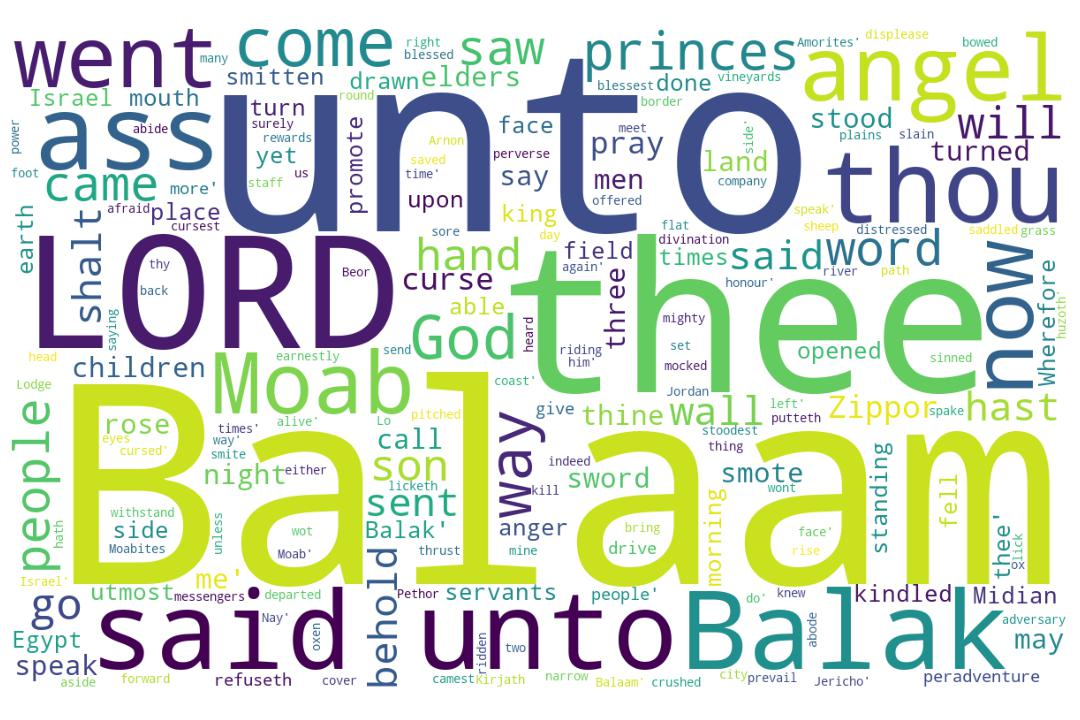
\includegraphics[width=\linewidth]{04OT-Numbers/Numbers22-WordCloud.jpg}
  \caption{Numbers 22 Word Cloud}
  \label{fig:Numbers 22 word Cloud}
\end{figure}

\marginpar{\scriptsize \centering \fcolorbox{bone}{lime}{\textbf{BALAAM'S RELIGION }}\\ (Numbers 22) \begin{compactenum}[I.][8]
    \item  \textbf{Assigned Diplomats} \index[scripture]{Numbers!Num 22:05}\index[scripture]{Numbers!Num 22:15} (Numbers 22:5, 15)
    \item  \textbf{Asking for Divination} \index[scripture]{Numbers!Num 22:07} (Numbers 22:7)
    \item Balaam's \textbf{Attempted Disobedience} \index[scripture]{Numbers!Num 22:19} (Numbers 22:19)
    \item \textbf{Armament Drawn} \index[scripture]{Numbers!Num 22:23}\index[scripture]{Numbers!Num 22:31} (Numbers 22:23, 31)
    \item The \textbf{Ass falls Down} \index[scripture]{Numbers!Num 22:27} (Numbers 22:27)
    \item An \textbf{Argument with a Donkey} \index[scripture]{Numbers!Num 22:29} (Numbers 22:29)
    \item An \textbf{Acquired Doctrine} \index[scripture]{Numbers!Num 23}\index[scripture]{Revelation!Rev 02:14} (Numbers 22, Revelation 2:14)
\end{compactenum}}

%%%%%%%%%%%%%%%%%%%%%%%%%%%%%%%%%%%%%
%%%%%%%%%%%%%%%%%%%%%%%%%%%%%%%%%%%%%
\footnote{\textcolor[rgb]{0.00,0.25,0.00}{\hyperlink{NumbersTOC}{Return to end of Table of Contents.}}}\footnote{\href{https://audiobible.com/bible/numbers_22.html}{\textcolor[cmyk]{0.99998,1,0,0}{Numbers 22 Audio}}}\textcolor[cmyk]{0.99998,1,0,0}{And the children of Israel set forward, and pitched in the plains of Moab on this side Jordan \emph{by} Jericho.}\\
\\
\P \textcolor[cmyk]{0.99998,1,0,0}{And Balak the son of Zippor saw all that Israel had done to the Amorites.}
[3] \textcolor[cmyk]{0.99998,1,0,0}{And Moab was sore afraid of the people, because they \emph{were} many: and Moab was distressed because of the children of Israel.}
[4] \textcolor[cmyk]{0.99998,1,0,0}{And Moab said unto the elders of Midian, Now shall this company lick up all \emph{that} \emph{are} round about us, as the ox licketh up the grass of the field. And Balak the son of Zippor \emph{was} king of the Moabites at that time.}
[5] \textcolor[cmyk]{0.99998,1,0,0}{He sent messengers therefore unto Balaam the son of Beor to Pethor, which \emph{is} by the river of the land of the children of his people, to call him, saying, Behold, there is a people come out from Egypt: behold, they cover the face of the earth, and they abide over against me:}
[6] \textcolor[cmyk]{0.99998,1,0,0}{Come now therefore, I pray thee, curse me this people; for they \emph{are} too mighty for me: peradventure I shall prevail, \emph{that} we may smite them, and \emph{that} I may drive them out of the land: for I wot that he whom thou blessest \emph{is} blessed, and he whom thou cursest is cursed.}
[7] \textcolor[cmyk]{0.99998,1,0,0}{And the elders of Moab and the elders of Midian departed with the rewards of divination in their hand; and they came unto Balaam, and spake unto him the words of Balak.}
[8] \textcolor[cmyk]{0.99998,1,0,0}{And he said unto them, Lodge here this night, and I will bring you word again, as the LORD shall speak unto me: and the princes of Moab abode with Balaam.}
[9] \textcolor[cmyk]{0.99998,1,0,0}{And God came unto Balaam, and said, What men \emph{are} these with thee?}
[10] \textcolor[cmyk]{0.99998,1,0,0}{And Balaam said unto God, Balak the son of Zippor, king of Moab, hath sent unto me, \emph{saying},}
[11] \textcolor[cmyk]{0.99998,1,0,0}{Behold, \emph{there} \emph{is} a people come out of Egypt, which covereth the face of the earth: come now, curse me them; peradventure I shall be able to overcome them, and drive them out.}
[12] \textcolor[cmyk]{0.99998,1,0,0}{And God said unto Balaam, Thou shalt not go with them; thou shalt not curse the people: for they \emph{are} blessed.}
[13] \textcolor[cmyk]{0.99998,1,0,0}{And Balaam rose up in the morning, and said unto the princes of Balak, Get you into your land: for the LORD refuseth to give me leave to go with you.}
[14] \textcolor[cmyk]{0.99998,1,0,0}{And the princes of Moab rose up, and they went unto Balak, and said, Balaam refuseth to come with us.}\\
\\
\P \textcolor[cmyk]{0.99998,1,0,0}{And Balak sent yet again princes, more, and more honourable than they.}
[16] \textcolor[cmyk]{0.99998,1,0,0}{And they came to Balaam, and said to him, Thus saith Balak the son of Zippor, Let nothing, I pray thee, hinder thee from coming unto me:}
[17] \textcolor[cmyk]{0.99998,1,0,0}{For I will promote thee unto very great honour, and I will do whatsoever thou sayest unto me: come therefore, I pray thee, curse me this people.}
[18] \textcolor[cmyk]{0.99998,1,0,0}{And Balaam answered and said unto the servants of Balak, If Balak would give me his house full of silver and gold, I cannot go beyond the word of the LORD my God, to do less or more.}
[19] \textcolor[cmyk]{0.99998,1,0,0}{Now therefore, I pray you, tarry ye also here this night, that I may know what the LORD will say unto me more.}
[20] \textcolor[cmyk]{0.99998,1,0,0}{And God came unto Balaam at night, and said unto him, If the men come to call thee, rise up, \emph{and} go with them; but yet the word which I shall say unto thee, that shalt thou do.}
[21] \textcolor[cmyk]{0.99998,1,0,0}{And Balaam rose up in the morning, and saddled his ass, and went with the princes of Moab.}\\
\\
\P  \textcolor[cmyk]{0.99998,1,0,0}{And God's anger was kindled because he went: and the angel of the LORD stood in the way for an adversary against him. Now he was riding upon his ass, and his two servants \emph{were} with him.}
[23] \textcolor[cmyk]{0.99998,1,0,0}{And the ass saw the angel of the LORD standing in the way, and his sword drawn in his hand: and the ass turned aside out of the way, and went into the field: and Balaam smote the ass, to turn her into the way.}
[24] \textcolor[cmyk]{0.99998,1,0,0}{But the angel of the LORD stood in a path of the vineyards, a wall \emph{being} on this side, and a wall on that side.}
[25] \textcolor[cmyk]{0.99998,1,0,0}{And when the ass saw the angel of the LORD, she thrust herself unto the wall, and crushed Balaam's foot against the wall: and he smote her again.}
[26] \textcolor[cmyk]{0.99998,1,0,0}{And the angel of the LORD went further, and stood in a narrow place, where \emph{was} no way to turn either to the right hand or to the left.}
[27] \textcolor[cmyk]{0.99998,1,0,0}{And when the ass saw the angel of the LORD, she fell down under Balaam: and Balaam's anger was kindled, and he smote the ass with a staff.}
[28] \textcolor[cmyk]{0.99998,1,0,0}{And the LORD opened the mouth of the ass, and she said unto Balaam, What have I done unto thee, that thou hast smitten me these three times?}
[29] \textcolor[cmyk]{0.99998,1,0,0}{And Balaam said unto the ass, Because thou hast mocked me: I would there were a sword in mine hand, for now would I kill thee.}
[30] \textcolor[cmyk]{0.99998,1,0,0}{And the ass said unto Balaam, \emph{Am} not I thine ass, upon which thou hast ridden ever since \emph{I} \emph{was} thine unto this day? was I ever wont to do so unto thee? And he said, Nay.}
[31] \textcolor[cmyk]{0.99998,1,0,0}{Then the LORD opened the eyes of Balaam, and he saw the angel of the LORD standing in the way, and his sword drawn in his hand: and he bowed down his head, and fell flat on his face.}
[32] \textcolor[cmyk]{0.99998,1,0,0}{And the angel of the LORD said unto him, Wherefore hast thou smitten thine ass these three times? behold, I went out to withstand thee, because \emph{thy} way is perverse before me:}
[33] \textcolor[cmyk]{0.99998,1,0,0}{And the ass saw me, and turned from me these three times: unless she had turned from me, surely now also I had slain thee, and saved her alive.}
[34] \textcolor[cmyk]{0.99998,1,0,0}{And Balaam said unto the angel of the LORD, I have sinned; for I knew not that thou stoodest in the way against me: now therefore, if it displease thee, I will get me back again.}
[35] \textcolor[cmyk]{0.99998,1,0,0}{And the angel of the LORD said unto Balaam, Go with the men: but only the word that I shall speak unto thee, that thou shalt speak. So Balaam went with the princes of Balak.}
[36] \textcolor[cmyk]{0.99998,1,0,0}{And when Balak heard that Balaam was come, he went out to meet him unto a city of Moab, which \emph{is} in the border of Arnon, which \emph{is} in the utmost coast.}
[37] \textcolor[cmyk]{0.99998,1,0,0}{And Balak said unto Balaam, Did I not earnestly send unto thee to call thee? wherefore camest thou not unto me? am I not able indeed to promote thee to honour?}
[38] \textcolor[cmyk]{0.99998,1,0,0}{And Balaam said unto Balak, Lo, I am come unto thee: have I now any power at all to say any thing? the word that God putteth in my mouth, that shall I speak.}
[39] \textcolor[cmyk]{0.99998,1,0,0}{And Balaam went with Balak, and they came unto Kirjath-huzoth.}
[40] \textcolor[cmyk]{0.99998,1,0,0}{And Balak offered oxen and sheep, and sent to Balaam, and to the princes that \emph{were} with him.}
[41] \textcolor[cmyk]{0.99998,1,0,0}{And it came to pass on the morrow, that Balak took Balaam, and brought him up into the high places of Baal, that thence he might see the utmost \emph{part} of the people.}
\chapter{Numbers 23}

%[cmyk]{0.99998,1,0,0}{

\marginpar{\scriptsize \centering \fcolorbox{bone}{lime}{\textbf{ATTEMPT TO CURSE ISRAEL}}\\ (Numbers 23)
\begin{compactenum}[I.][8]
   \item A \textbf{Nation set Apart} \index[scripture]{Numbers!Num 23:09} (Numbers 23:9)
    \item A \textbf{Nation Protected} \index[scripture]{Numbers!Num 23:09} (Numbers 23:9)
    \item A \textbf{Nation Preferred} \index[scripture]{Numbers!Num 23:09} (Numbers 23:9)
    \item A \textbf{Notable Parable} \index[scripture]{Numbers!Num 23:07} (Numbers 23:7)
    \item A \textbf{Notion that is Poisonous} (to prefer what God prefers) \index[scripture]{Numbers!Num 23:11} (Numbers 23:11)
    \item The \textbf{Nagging Problem} \index[scripture]{Numbers!Num 23:12} (Numbers 23:12)
    \begin{compactenum}[A.][8]
    	\item Balak could not get the solution he wanted, despite co--opting religion
        \item Israel holds a special and protected place, a place enforced by God Himself.
        \item Cannot curse what God has blessed
    \end{compactenum}\end{compactenum}}
    
%%%%%%%%%%%%%%%%%%%%%%%%%%%%%%%%%%%%%%%%
%%%%%%%%%%%%%%%%%%%%%%%%%%%%%%%%%%%%%%%%
\footnote{\textcolor[rgb]{0.00,0.25,0.00}{\hyperlink{NumbersTOC}{Return to end of Table of Contents.}}}\footnote{\href{https://audiobible.com/bible/numbers_23.html}{\textcolor[cmyk]{0.99998,1,0,0}{Numbers 23 Audio}}}\textcolor[cmyk]{0.99998,1,0,0}{And \fcolorbox{bone}{bone}{Balaam} said unto Balak, Build me here seven altars, and prepare me here seven oxen and seven rams.}
[2] \textcolor[cmyk]{0.99998,1,0,0}{And Balak did as \fcolorbox{bone}{bone}{Balaam} had spoken; and Balak and \fcolorbox{bone}{bone}{Balaam} offered on \emph{every} altar a bullock and a ram.}
[3] \textcolor[cmyk]{0.99998,1,0,0}{And \fcolorbox{bone}{bone}{Balaam} said unto Balak, Stand by thy burnt offering, and I will go: peradventure the LORD will come to meet me: and whatsoever he sheweth me I will tell thee. And he went to an high place.}
[4] \textcolor[cmyk]{0.99998,1,0,0}{And God met \fcolorbox{bone}{bone}{Balaam}: and he said unto him, I have prepared seven altars, and I have offered upon \emph{every} altar a bullock and a ram.}
[5] \textcolor[cmyk]{0.99998,1,0,0}{And the LORD put a word in Balaam's mouth, and said, Return unto Balak, and thus thou shalt speak.}
[6] \textcolor[cmyk]{0.99998,1,0,0}{And he returned unto him, and, lo, he stood by his burnt sacrifice, he, and all the princes of Moab.}
[7] \textcolor[cmyk]{0.99998,1,0,0}{And he took up his parable, and said, Balak the king of Moab hath brought me from Aram, out of the mountains of the east, \emph{saying}, Come, curse me Jacob, and come, defy Israel.}
[8] \textcolor[cmyk]{0.99998,1,0,0}{How shall I curse, whom God hath not cursed? or how shall I defy, \emph{whom} the LORD hath not defied?}
[9] \textcolor[cmyk]{0.99998,1,0,0}{For from the top of the rocks I see him, and from the hills I behold him: lo, the people shall dwell alone, and shall not be reckoned among the nations.}
[10] \textcolor[cmyk]{0.99998,1,0,0}{Who can count the dust of Jacob, and the number of the fourth \emph{part} of Israel? Let me die the death of the righteous, and let my last end be like his!}
[11] \textcolor[cmyk]{0.99998,1,0,0}{And Balak said unto \fcolorbox{bone}{bone}{Balaam}, What hast thou done unto me? I took thee to curse mine enemies, and, behold, thou hast blessed \emph{them} altogether.}
[12] \textcolor[cmyk]{0.99998,1,0,0}{And he answered and said, Must I not take heed to speak that which the LORD hath put in my mouth?}
[13] \textcolor[cmyk]{0.99998,1,0,0}{And Balak said unto him, Come, I pray thee, with me unto another place, from whence thou mayest see them: thou shalt see but the utmost part of them, and shalt not see them all: and curse me them from thence.}\\
\\
\P \textcolor[cmyk]{0.99998,1,0,0}{And he brought him into the field of Zophim, to the top of Pisgah, and built seven altars, and offered a bullock and a ram on \emph{every} altar.}
[15] \textcolor[cmyk]{0.99998,1,0,0}{And he said unto Balak, Stand here by thy burnt offering, while I meet \emph{the} \emph{LORD} yonder.}
[16] \textcolor[cmyk]{0.99998,1,0,0}{And the LORD met \fcolorbox{bone}{bone}{Balaam}, and put a word in his mouth, and said, Go again unto Balak, and say thus.}
[17] \textcolor[cmyk]{0.99998,1,0,0}{And when he came to him, behold, he stood by his burnt offering, and the princes of Moab with him. And Balak said unto him, What hath the LORD spoken?}
[18] \textcolor[cmyk]{0.99998,1,0,0}{And he took up his parable, and said, Rise up, Balak, and hear; hearken unto me, thou son of Zippor:}
[19] \textcolor[cmyk]{0.99998,1,0,0}{God \emph{is} not a man, that he should lie; neither the son of man, that he should repent: hath he said, and shall he not do \emph{it}? or hath he spoken, and shall he not make it good?}
[20] \textcolor[cmyk]{0.99998,1,0,0}{Behold, I have received \emph{commandment} to bless: and he hath blessed; and I cannot reverse it.}
[21] \textcolor[cmyk]{0.99998,1,0,0}{He hath not beheld iniquity in Jacob, neither hath he seen perverseness in Israel: the LORD his God \emph{is} with him, and the shout of a king \emph{is} among them.}
[22] \textcolor[cmyk]{0.99998,1,0,0}{God brought them out of Egypt; he hath as it were the strength of an unicorn.}
[23] \textcolor[cmyk]{0.99998,1,0,0}{Surely \emph{there} \emph{is} no enchantment against Jacob, neither \emph{is} \emph{there} any divination against Israel: according to this time it shall be said of Jacob and of Israel, What hath God wrought!}
[24] \textcolor[cmyk]{0.99998,1,0,0}{Behold, the people shall rise up as a great lion, and lift up himself as a young lion: he shall not lie down until he eat \emph{of} the prey, and drink the blood of the slain.}\\
\\
\P \textcolor[cmyk]{0.99998,1,0,0}{And Balak said unto \fcolorbox{bone}{bone}{Balaam}, Neither curse them at all, nor bless them at all.}
[26] \textcolor[cmyk]{0.99998,1,0,0}{But \fcolorbox{bone}{bone}{Balaam} answered and said unto Balak, Told not I thee, saying, All that the LORD speaketh, that I must do?}\\
\\
\P \textcolor[cmyk]{0.99998,1,0,0}{And Balak said unto \fcolorbox{bone}{bone}{Balaam}, Come, I pray thee, I will bring thee unto another place; peradventure it will please God that thou mayest curse me them from thence.}
[28] \textcolor[cmyk]{0.99998,1,0,0}{And Balak brought \fcolorbox{bone}{bone}{Balaam} unto the top of Peor, that looketh toward Jeshimon.}
[29] \textcolor[cmyk]{0.99998,1,0,0}{And \fcolorbox{bone}{bone}{Balaam} said unto Balak, Build me here seven altars, and prepare me here seven bullocks and seven rams.}
[30] \textcolor[cmyk]{0.99998,1,0,0}{And Balak did as \fcolorbox{bone}{bone}{Balaam} had said, and offered a bullock and a ram on \emph{every} altar.}
\chapter{Numbers 24}

\begin{figure}
  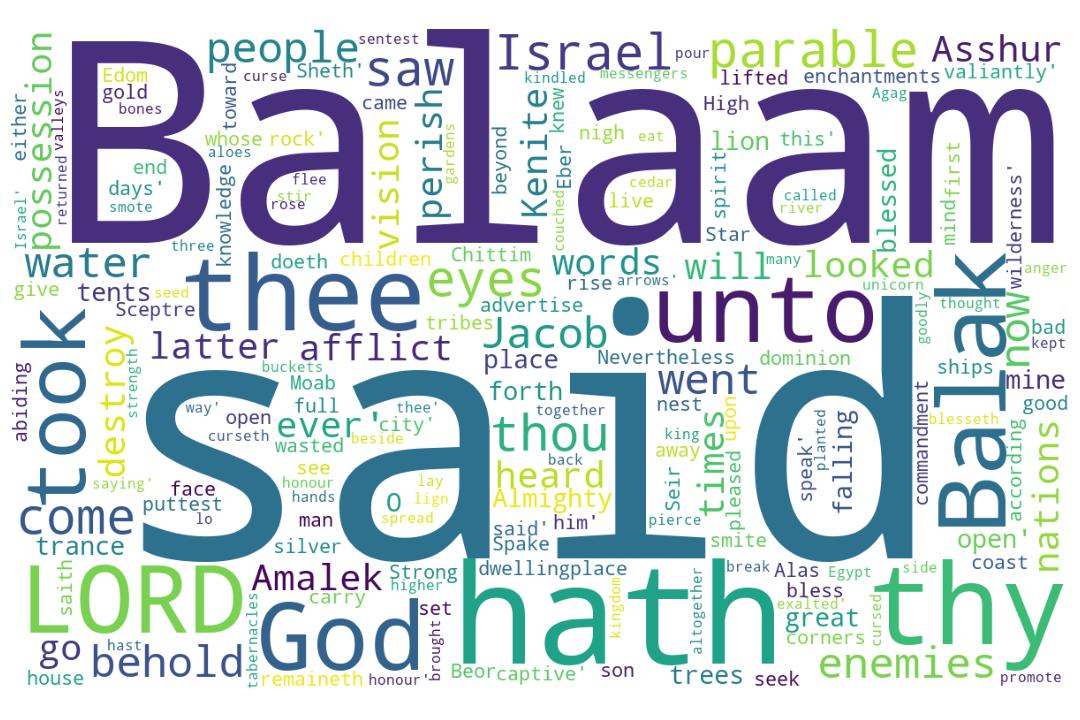
\includegraphics[width=\linewidth]{04OT-Numbers/Numbers24-WordCloud.jpg}
  \caption{Numbers 24 Word Cloud}
  \label{fig:Numbers 24 word Cloud}
\end{figure}

\marginpar{\scriptsize \centering \fcolorbox{bone}{lime}{\textbf{BALAAM'S MINISTRY}}\\ (Numbers 24)
\begin{compactenum}[I.][8]
    \item His \textbf{Compromise} \index[scripture]{Numbers!Num 31:16} (Numbers 31:16) (we find out in Numbers 31 what Balaam's advice was to Balam. The advice is followed in Numbers 25.)
    \item His \textbf{Consideration} \index[scripture]{Numbers!Num 24:01} (Numbers 24:1) 
    \item His \textbf{Coins} \index[scripture]{Jude!Jde 1:11} (Jude 1:11) (his reward)
    \item His \textbf{Corruption} %\index[scripture]{Jude!Jde 1:11} (Jude 1:11) (his reward)
    \item His \textbf{Counsel} \index[scripture]{Numbers!Num 25:03} \index[scripture]{Revelation!Rev 02:14} (Numbers 25:3, Revelation 2:14) (defeat Israel by corrupting them. This happens with the worship of Baal-Peor in Numbers 25. We likely see parallel examples in 21$^{st}$-century Christianity.)
\end{compactenum}}

%%%%%%%%%%%%%%%%%%%%%%%%%%%%%%%%%%
%%%%%%%%%%%%%%%%%%%%%%%%%%%%%%%%%%
\footnote{\textcolor[rgb]{0.00,0.25,0.00}{\hyperlink{NumbersTOC}{Return to end of Table of Contents.}}}\footnote{\href{https://audiobible.com/bible/numbers_24.html}{\textcolor[cmyk]{0.99998,1,0,0}{Numbers 24 Audio}}}\textcolor[cmyk]{0.99998,1,0,0}{\fcolorbox{bone}{bone}{And} when Balaam saw that it pleased the LORD to bless Israel, he went not, as at other times, to seek for enchantments, but he set his face toward the wilderness.}
[2] \textcolor[cmyk]{0.99998,1,0,0}{\fcolorbox{bone}{bone}{And} Balaam lifted up his eyes, and he saw Israel abiding \emph{in} \emph{his} \emph{tents} according to their tribes; and the spirit of God came upon him.}
[3] \textcolor[cmyk]{0.99998,1,0,0}{\fcolorbox{bone}{bone}{And} he took up his parable, and \fcolorbox{bone}{bone}{said}, Balaam the son of Beor hath \fcolorbox{bone}{bone}{said}, and the man whose eyes are open hath \fcolorbox{bone}{bone}{said}:}
[4] \textcolor[cmyk]{0.99998,1,0,0}{He hath \fcolorbox{bone}{bone}{said}, which heard the words of God, which saw the vision of the Almighty, falling \emph{into} \emph{a} \emph{trance}, but having his eyes open:}
[5] \textcolor[cmyk]{0.99998,1,0,0}{How goodly are thy tents, O Jacob, \emph{and} thy tabernacles, O Israel!}
[6] \textcolor[cmyk]{0.99998,1,0,0}{As the valleys are they spread forth, as gardens by the river's side, as the trees of lign aloes which the LORD hath planted, \emph{and} as cedar trees beside the waters.}
[7] \textcolor[cmyk]{0.99998,1,0,0}{He shall pour the water out of his buckets, and his seed \emph{shall} \emph{be} in many waters, and his king shall be higher than Agag, and his kingdom shall be exalted.}
[8] \textcolor[cmyk]{0.99998,1,0,0}{God brought him forth out of Egypt; he hath as it were the strength of an unicorn: he shall eat up the nations his enemies, and shall break their bones, and pierce \emph{them} through with his arrows.}
[9] \textcolor[cmyk]{0.99998,1,0,0}{He couched, he lay down as a lion, and as a great lion: who shall stir him up? Blessed \emph{is} he that blesseth thee, and cursed \emph{is} he that curseth thee.}\\
\\
\P \textcolor[cmyk]{0.99998,1,0,0}{\fcolorbox{bone}{bone}{And} Balak's anger was kindled against Balaam, and he smote his hands together: and Balak \fcolorbox{bone}{bone}{said} unto Balaam, I called thee to curse mine enemies, and, behold, thou hast altogether blessed \emph{them} these three times.}
[11] \textcolor[cmyk]{0.99998,1,0,0}{Therefore now flee thou to thy place: I thought to promote thee unto great honour; but, lo, the LORD hath kept thee back from honour.}
[12] \textcolor[cmyk]{0.99998,1,0,0}{\fcolorbox{bone}{bone}{And} Balaam \fcolorbox{bone}{bone}{said} unto Balak, Spake I not also to thy messengers which thou sentest unto me, saying,}
[13] \textcolor[cmyk]{0.99998,1,0,0}{If Balak would give me his house full of silver and gold, I cannot go beyond the commandment of the LORD, to do \emph{either} good or bad of mine own mind; \emph{but} what the LORD saith, that will I speak?}
[14] \textcolor[cmyk]{0.99998,1,0,0}{\fcolorbox{bone}{bone}{And} now, behold, I go unto my people: come \emph{therefore,} \emph{and} I will advertise thee what this people shall do to thy people in the latter days.}\\
\\
\P \textcolor[cmyk]{0.99998,1,0,0}{\fcolorbox{bone}{bone}{And} he took up his parable, and \fcolorbox{bone}{bone}{said}, Balaam the son of Beor hath \fcolorbox{bone}{bone}{said}, and the man whose eyes are open hath \fcolorbox{bone}{bone}{said}:}
[16] \textcolor[cmyk]{0.99998,1,0,0}{He hath \fcolorbox{bone}{bone}{said}, which heard the words of God, and knew the knowledge of the most High, \emph{which} saw the vision of the Almighty, falling \emph{into} \emph{a} \emph{trance}, but having his eyes open:}
[17] \textcolor[cmyk]{0.99998,1,0,0}{I shall see him, but not now: I shall behold him, but not nigh: there shall come a Star out of Jacob, and a Sceptre shall rise out of Israel, and shall smite the corners of Moab, and destroy all the children of Sheth.}
[18] \textcolor[cmyk]{0.99998,1,0,0}{\fcolorbox{bone}{bone}{And} Edom shall be a possession, Seir also shall be a possession for his enemies; and Israel shall do valiantly.}
[19] \textcolor[cmyk]{0.99998,1,0,0}{Out of Jacob shall come he that shall have dominion, and shall destroy him that remaineth of the city.}\\
\\
\P \textcolor[cmyk]{0.99998,1,0,0}{\fcolorbox{bone}{bone}{And} when he looked on Amalek, he took up his parable, and \fcolorbox{bone}{bone}{said}, Amalek \emph{was} the first of the nations; but his latter end \emph{shall} \emph{be} that he perish for ever.}
[21] \textcolor[cmyk]{0.99998,1,0,0}{\fcolorbox{bone}{bone}{And} he looked on the Kenites, and took up his parable, and \fcolorbox{bone}{bone}{said}, Strong is thy \fcolorbox{bone}{MYGOLD}{dwellingplace}, and thou puttest thy nest in a rock.}
[22] \textcolor[cmyk]{0.99998,1,0,0}{Nevertheless the Kenite shall be wasted, until Asshur shall carry thee away captive.}
[23] \textcolor[cmyk]{0.99998,1,0,0}{\fcolorbox{bone}{bone}{And} he took up his parable, and \fcolorbox{bone}{bone}{said}, Alas, who shall live when God doeth this!}
[24] \textcolor[cmyk]{0.99998,1,0,0}{\fcolorbox{bone}{bone}{And} ships \emph{shall} \emph{come} from the coast of Chittim, and shall afflict Asshur, and shall afflict Eber, and he also shall perish for ever.}
[25] \textcolor[cmyk]{0.99998,1,0,0}{\fcolorbox{bone}{bone}{And} Balaam rose up, and went and returned to his place: and Balak also went his way.}

\chapter{Psalm 48}

\begin{figure}
  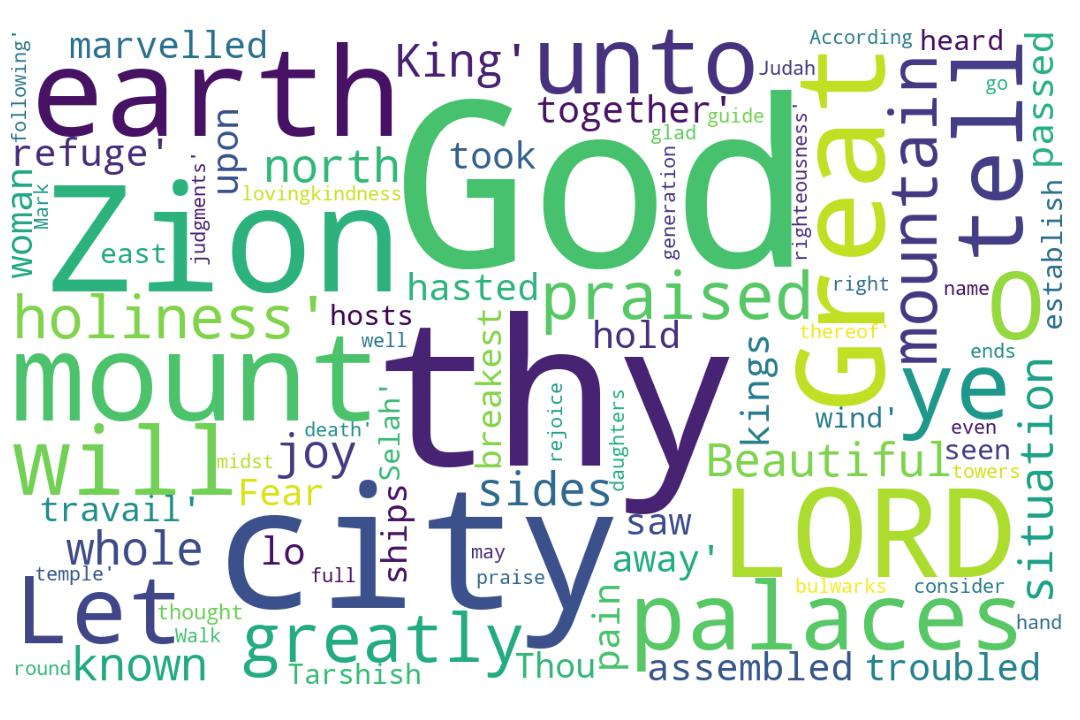
\includegraphics[width=\linewidth]{19OT-Psalms/Psalm48-WordCloud.jpg}
  \caption{Psalm 48 Word Cloud}
  \label{fig:Psalm 48 word Cloud}
\end{figure}



\marginpar{\scriptsize \centering \fcolorbox{bone}{lime}{\textbf{GOD, HIS THRONE, HIS CITY}}\\ (Psalm 48:1-14) \begin{compactenum}[I.][8]
    \item His \textbf{Greatness} \index[scripture]{Psalms!Psa 048:01}(Psa 48:1)
    \item His \textbf{Geography} \index[scripture]{Psalms!Psa 048:02}(Psa 48:2)
    \item Our \textbf{Refuge} \index[scripture]{Psalms!Psa 048:03}(Psa 48:3)
    \item His \textbf{Goodness} \index[scripture]{Psalms!Psa 048:09}(Psa 48:9)
    \item Our \textbf{Gladness} \index[scripture]{Psalms!Psa 048:11}(Psa 48:11)
    \item His \textbf{Glorification} \index[scripture]{Psalms!Psa 048:10}(Psa 48:10)
    \item Our \textbf{Guide} \index[scripture]{Psalms!Psa 048:14}(Psa 48:14)
\end{compactenum}}
    
%%%%%%%%%%%%%%%%%%%%%%%%%%%%%%
%%%%%%%%%%%%%%%%%%%%%%%%%%%%%%
\footnote{\textcolor[cmyk]{0.99998,1,0,0}{\hyperlink{TOC}{Return to end of Table of Contents.}}}\footnote{\href{https://audiobible.com/bible/psalms_48.html}{\textcolor[cmyk]{0.99998,1,0,0}{Psalms Audio}}}\textcolor[cmyk]{0.99998,1,0,0}{A Song \emph{and} Psalm for the sons of Korah.}\\
\\
\textcolor[cmyk]{0.99998,1,0,0}{\fcolorbox{bone}{lime}{Great} \emph{is} the LORD, and greatly to be praised in the city of our God, \emph{in} the mountain of his holiness.}
[2] \textcolor[cmyk]{0.99998,1,0,0}{Beautiful for situation, the joy of the \fcolorbox{bone}{lime}{whole earth}, \emph{is} mount Zion, \emph{on} the sides of the north, the city of the great King.}
[3] \textcolor[cmyk]{0.99998,1,0,0}{God is known in her palaces for a \fcolorbox{bone}{lime}{refuge}.}
[4] \textcolor[cmyk]{0.99998,1,0,0}{For, lo, the kings were assembled, they passed by together.}
[5] \textcolor[cmyk]{0.99998,1,0,0}{They saw \emph{it,} \emph{and} so they marvelled; they were troubled, \emph{and} hasted away.}
[6] \textcolor[cmyk]{0.99998,1,0,0}{Fear took hold upon them there, \emph{and} pain, as of a woman in travail.}
[7] \textcolor[cmyk]{0.99998,1,0,0}{Thou breakest the ships of Tarshish with an east wind.}
[8] \textcolor[cmyk]{0.99998,1,0,0}{As we have heard, so have we seen in the city of the LORD of hosts, in the city of our God: God will establish it for ever. Selah.}
[9] \textcolor[cmyk]{0.99998,1,0,0}{We have thought of thy \fcolorbox{bone}{lime}{lovingkindness}, O God, in the midst of thy temple.}
[10] \textcolor[cmyk]{0.99998,1,0,0}{According to thy name, O God, so \emph{is} thy \fcolorbox{bone}{lime}{praise} unto the ends of the earth: thy right hand is full of \fcolorbox{bone}{MYGOLD}{righteousness}.}
[11] \textcolor[cmyk]{0.99998,1,0,0}{Let mount Zion rejoice, let the daughters of Judah be \fcolorbox{bone}{lime}{glad}, because of thy judgments.}
[12] \textcolor[cmyk]{0.99998,1,0,0}{Walk about Zion, and go round about her: tell the towers thereof.}
[13] \textcolor[cmyk]{0.99998,1,0,0}{Mark ye well her bulwarks, consider her palaces; that ye may tell \emph{it} to the generation following.}
[14] \textcolor[cmyk]{0.99998,1,0,0}{For this God \emph{is} our God for ever and ever: he will be our \fcolorbox{bone}{lime}{guide} \emph{even} unto death.}

\chapter{Proverb 17}
\begin{figure}
  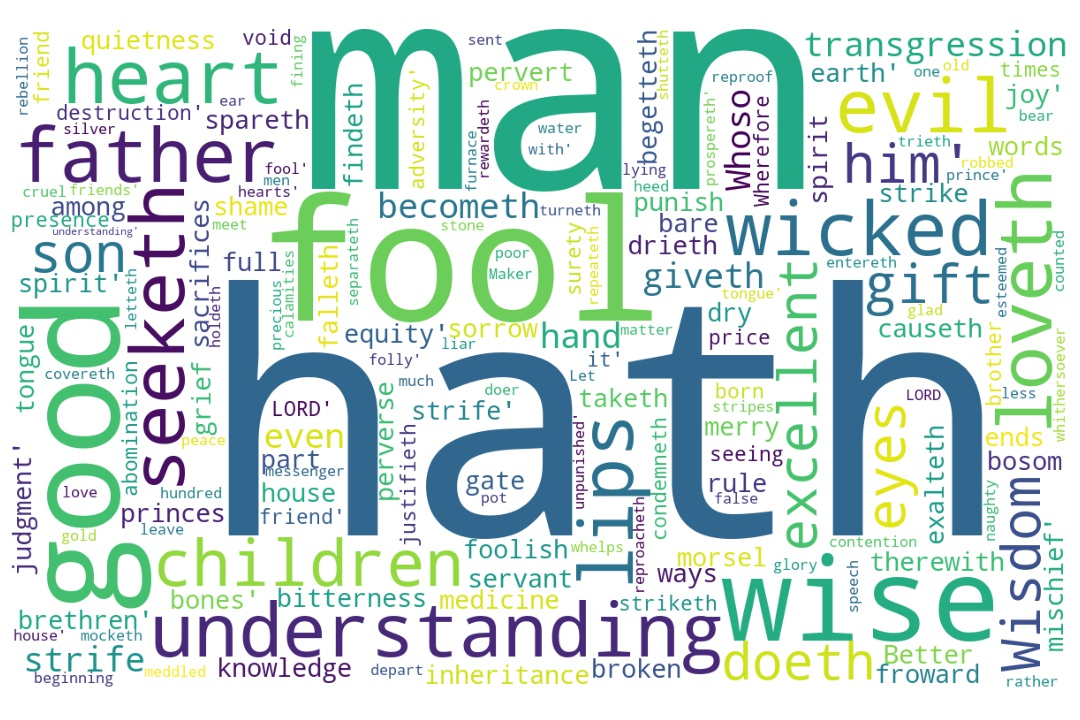
\includegraphics[width=\linewidth]{20OT-Proverbs/Proverb17-WordCloud.jpg}
  \caption{Proverb 17 Word Cloud}
  \label{fig:Proverb 17 word Cloud}
\end{figure}

\marginpar{\scriptsize \centering \fcolorbox{bone}{lime}{\textbf{CONTRASTS}}\\ (Proverbs 17:1-28) \begin{compactenum}[I.][8]
    \item \textbf{A Dry Morsel} \index[scripture]{Proverbs!Pro 17:01}(Pro 17:1) 
    \item \textbf{A Dim-Witted Mocker} \index[scripture]{Proverbs!Pro 17:05}(Pro 17:5) 
    \item \textbf{A Divisive Matter} \index[scripture]{Proverbs!Pro 17:09}(Pro 17:9) 
    \item \textbf{A Disruptive Messenger} \index[scripture]{Proverbs!Pro 17:11}(Pro 17:11) 
    \item \textbf{Destructive Meddling} \index[scripture]{Proverbs!Pro 17:14}(Pro 17:14) 
    \item \textbf{Dangerous Mischief} \index[scripture]{Proverbs!Pro 17:20}(Pro 17:20) 
    \item \textbf{A Discerning Man} \index[scripture]{Proverbs!Pro 17:28} (Pro 17:28) 
\end{compactenum} }

\marginpar{\scriptsize \centering \fcolorbox{bone}{yellow}{\textbf{THE FRUIT OF FOOLS}}\\ (Proverbs 17:1-28) \begin{compactenum}[I.][8]
    \item \textbf{Unwanted Family} \index[scripture]{Proverbs!Pro 17:01}(Pro 17:1) 
    \item \textbf{Unteachable Fool} \index[scripture]{Proverbs!Pro 17:10}(Pro 17:10) 
    \item \textbf{Unstoppable Fool} \index[scripture]{Proverbs!Pro 17:11}(Pro 17:11)  
    \item \textbf{Unrestrained Fanatic} \index[scripture]{Proverbs!Pro 17:11}(Pro 17:11)
    \item \textbf{Uncontrollable Flood} \index[scripture]{Proverbs!Pro 17:14}(Pro 17:14)  
    \item \textbf{Unshakeable Fealty} \index[scripture]{Proverbs!Pro 17:17}(Pro 17:17)  
    \item \textbf{Unfulfilled Father} \index[scripture]{Proverbs!Pro 17:21}(Pro 17:21) 
    \item \textbf{Unobtainable Focus} \index[scripture]{Proverbs!Pro 17:24}(Pro 17:24)  
\end{compactenum} }

\footnote{\textcolor[cmyk]{0.99998,1,0,0}{\hyperlink{TOC}{Return to end of Table of Contents.}}}\footnote{\href{https://audiobible.com/bible/proverbs_17.html}{\textcolor[cmyk]{0.99998,1,0,0}{Proverbs Audio}}}\textcolor[cmyk]{0.99998,1,0,0}{Better \emph{is} a \fcolorbox{bone}{lime}{dry morsel}, and quietness therewith, than an house full of sacrifices \emph{with} strife.}
[2] \textcolor[cmyk]{0.99998,1,0,0}{A wise servant shall have rule over a son that causeth shame, and shall have part of the inheritance among the brethren.}
[3] \textcolor[cmyk]{0.99998,1,0,0}{The fining pot \emph{is} for silver, and the furnace for gold: but the LORD trieth the hearts.}
[4] \textcolor[cmyk]{0.99998,1,0,0}{A wicked doer giveth heed to false lips; \emph{and} a liar giveth ear to a naughty tongue.}
[5] \textcolor[cmyk]{0.99998,1,0,0}{Whoso \fcolorbox{bone}{lime}{mocketh} the poor reproacheth his Maker: \emph{and} he that is glad at calamities shall not be unpunished.}
[6] \textcolor[cmyk]{0.99998,1,0,0}{Children's children \emph{are} the crown of old men; and the glory of children \emph{are} their fathers.}
[7] \textcolor[cmyk]{0.99998,1,0,0}{Excellent speech becometh not a fool: much less do lying lips a prince.}
[8] \textcolor[cmyk]{0.99998,1,0,0}{A gift \emph{is} \emph{as} a precious stone in the eyes of him that hath it: \fcolorbox{bone}{MYGOLD}{whithersoever} it turneth, it prospereth.}
[9] \textcolor[cmyk]{0.99998,1,0,0}{He that covereth a \fcolorbox{bone}{MYGOLD}{transgression} seeketh love; but he that repeateth a matter \fcolorbox{bone}{lime}{separateth} \emph{very} friends.}
[10] \textcolor[cmyk]{0.99998,1,0,0}{A reproof entereth more into a wise man than an hundred stripes into a fool.}
[11] \textcolor[cmyk]{0.99998,1,0,0}{An evil \emph{man} seeketh only rebellion: therefore a \fcolorbox{bone}{lime}{cruel messenger} shall be sent against him.}
[12] \textcolor[cmyk]{0.99998,1,0,0}{Let a bear robbed of her whelps meet a man, rather than a fool in his folly.}
[13] \textcolor[cmyk]{0.99998,1,0,0}{Whoso rewardeth evil for good, evil shall not depart from his house.}
[14] \textcolor[cmyk]{0.99998,1,0,0}{The beginning of strife \emph{is} \emph{as} when one letteth out water: therefore leave off contention, before it be \fcolorbox{bone}{lime}{meddled} with.}
[15] \textcolor[cmyk]{0.99998,1,0,0}{He that justifieth the wicked, and he that condemneth the just, even they both \emph{are} abomination to the LORD.}
[16] \textcolor[cmyk]{0.99998,1,0,0}{Wherefore \emph{is} \emph{there} a price in the hand of a fool to get wisdom, seeing \emph{he} \emph{hath} no heart \emph{to} \emph{it}?}
[17] \textcolor[cmyk]{0.99998,1,0,0}{A friend loveth at all times, and a brother is born for adversity.}
[18] \textcolor[cmyk]{0.99998,1,0,0}{A man void of \fcolorbox{bone}{MYGOLD}{understanding} striketh hands, \emph{and} becometh surety in the presence of his friend.}
[19] \textcolor[cmyk]{0.99998,1,0,0}{He loveth \fcolorbox{bone}{MYGOLD}{transgression} that loveth strife: \emph{and} he that exalteth his gate seeketh destruction.}
[20] \textcolor[cmyk]{0.99998,1,0,0}{He that hath a froward heart findeth no good: and he that hath a perverse tongue falleth into \fcolorbox{bone}{lime}{mischief}.}
[21] \textcolor[cmyk]{0.99998,1,0,0}{He that begetteth a fool \emph{doeth} \emph{it} to his sorrow: and the father of a fool hath no joy.}
[22] \textcolor[cmyk]{0.99998,1,0,0}{A merry heart doeth good \emph{like} a medicine: but a broken spirit drieth the bones.}
[23] \textcolor[cmyk]{0.99998,1,0,0}{A wicked \emph{man} taketh a gift out of the bosom to pervert the ways of judgment.}
[24] \textcolor[cmyk]{0.99998,1,0,0}{Wisdom \emph{is} before him that hath \fcolorbox{bone}{MYGOLD}{understanding}; but the eyes of a fool \emph{are} in the ends of the earth.}
[25] \textcolor[cmyk]{0.99998,1,0,0}{A foolish son \emph{is} a grief to his father, and bitterness to her that bare him.}
[26] \textcolor[cmyk]{0.99998,1,0,0}{Also to punish the just \emph{is} not good, \emph{nor} to strike princes for equity.}
[27] \textcolor[cmyk]{0.99998,1,0,0}{He that hath knowledge spareth his words: \emph{and} a man of \fcolorbox{bone}{MYGOLD}{understanding} is of an excellent spirit.}
[28] \textcolor[cmyk]{0.99998,1,0,0}{Even a fool, when he holdeth his peace, is counted wise: \emph{and} he that shutteth his lips \emph{is} \emph{esteemed} \fcolorbox{bone}{lime}{a man of \fcolorbox{bone}{MYGOLD}{understanding}}.}




\end{document}

